\documentclass[sectionformat = aufgabe]{gadsescript}

\usepackage{pgfplots}
\pgfplotsset{compat=1.18}

\defaulttitleh
\settitle{Übungsblatt Nr. 3}
\setsubtitle{Jörg und Elias}
\setfaculty{Faculty of Science (Physics)}

\begin{document}
\maketitle

\section{Newtonsche Reibung}
\begin{enumerate}[label=\alph*)]
	\item $ F_{ges} = F_g + \kappa v^2 $
	\item für die Endgeschwindigkeit gilt $ a = \qty{0}{\metre\per\square\second} $, also
		\begin{align*}
			F_{ges} &= \qty{0}{\kilogram\metre\per\square\second}\\
			F_g + \kappa v_{\infty}^2 &= \qty{0}{\kilogram\metre\per\square\second}\\
			\kappa v_\infty^2 &= -F_g\\
			v^2 &= -\frac{F_g}{\kappa}\\
			|v_\infty| &= \sqrt{-\frac{F_g}{\kappa}}
		\end{align*}
	\item $ u \coloneqq \sqrt{-\frac{\kappa}{F_g}} v, \xi \coloneqq \sqrt{-\frac{m}{4\kappa a}}, \tau \coloneqq u - 1, \vartheta \coloneqq u + 1 $, daraus folgt:\\
		$ v = \sqrt{-\frac{F_g}{\kappa}}, dv = \sqrt{-\frac{\kappa}{F_g}} du, du = d\tau, du = d\vartheta $
		Es gilt:
		\begin{align*}
			F_{ges} &= F_g + \kappa v^2\\
			m \frac{dv}{dt} &= F_g + \kappa v^2\\
			dt &= \frac{m}{F_g + \kappa v^2} dv &&| \text{ Substitution}\\
			dt &= \frac{m}{F_g ( 1 - u^2)} \sqrt{-\frac{F_g}{\kappa}} du\\
			dt &=  \sqrt{-\frac{m}{4\kappa a}} \cdot \frac{2}{ 1 - u^2} du\\
			dt &=  \xi \cdot \frac{2}{u^2 - 1} du\\
			\frac{1}{x}dt &=  \cdot \frac{2}{u^2 - 1} du\\
		\end{align*}
		Da
		\begin{align*}
			\frac{1}{\tau} d\tau - \frac{1}{\vartheta}d\vartheta &= \frac{1}{u - 1}du - \frac{1}{u + 1}du\\
			~&= \left(\frac{1}{u - 1} - \frac{1}{u + 1}\right)du\\
			~&= \left(\frac{u + 1  - (u - 1)}{(u - 1) (u + 1)}\right)du\\
			~&= \frac{2}{u^2 - 1}du
		\end{align*}
		gilt:
		\begin{align*}
			\frac{1}{\xi}dt &= \frac{2}{u^2 - 1} du\\
			\frac{1}{\xi}dt &= \frac{1}{\tau} d\tau - \frac{1}{\vartheta}d\vartheta\\
			\int_{t_0}^{t_1} \frac{1}{\xi}dt &= \int_{\tau_0}^{\tau_1} \frac{1}{\tau} d\tau - \int_{\vartheta_0}^{\vartheta_1} \frac{1}{\vartheta}d\vartheta\\
			\frac{1}{\xi} t &= \ln |\tau_1| - \ln |\tau_0| - \left( \ln |\vartheta_1| - \ln |\vartheta_0| \right)
		\end{align*}
		Durch Rücksubstituieren erhält man:
		\begin{align*}
			\frac{1}{\xi} t &= \ln |u_1 - 1| - \ln |u_0 - 1| - \left( \ln |u_1 + 1| - \ln |u_0 + 1| \right)\\
			\frac{1}{\xi} t &= \ln |\sqrt{-\frac{\kappa}{F_g}} v_1 - 1| - \ln |\underbrace{\sqrt{-\frac{\kappa}{F_g}} v_0}_{=0} - 1|\\
			~&\phantom{=} - \left( \ln |\sqrt{-\frac{\kappa}{F_g}} v_1 + 1| - \ln |\underbrace{\sqrt{-\frac{\kappa}{F_g}} v_0}_{=0} + 1| \right)\\
			\frac{1}{\xi} t &= \ln |\sqrt{-\frac{\kappa}{F_g}} v_1 - 1| - \ln |-1| - \left( \ln |\sqrt{-\frac{\kappa}{F_g}} v_1 + 1| - \ln |1| \right)\\
			\frac{1}{\xi} t &= \ln |\sqrt{-\frac{\kappa}{F_g}} v_1 - 1| - 0 - \left( \ln |\sqrt{-\frac{\kappa}{F_g}} v_1 + 1| - 0 \right)\\
			\frac{1}{\xi} t &= \ln |\sqrt{-\frac{\kappa}{F_g}} v_1 - 1|  - \ln |\sqrt{-\frac{\kappa}{F_g}} v_1 + 1|\\
			\frac{1}{\xi} t &= \ln \frac{|\sqrt{-\frac{\kappa}{F_g}} v_1 - 1|}{|\sqrt{-\frac{\kappa}{F_g}} v_1 + 1|}\\
			- \frac{1}{\xi} t &= \ln \frac{|\sqrt{-\frac{\kappa}{F_g}} v_1 + 1|}{|\sqrt{-\frac{\kappa}{F_g}} v_1 - 1|}\\
			\exp(- \frac{1}{\xi} t) &= \frac{|\sqrt{-\frac{\kappa}{F_g}} v_1 + 1|}{|\sqrt{-\frac{\kappa}{F_g}} v_1 - 1|}\\
			\exp(- \frac{1}{\xi} t) &= \frac{| v_1 + \sqrt{-\frac{F_g}{\kappa}}|}{| v_1 - \sqrt{-\frac{F_g}{\kappa}}|}
		\end{align*}
		Nach der b) ist $ |v_1| <= \sqrt{-\frac{F_g}{\kappa}} $ und da $a <= 0 $, also $ -v_1 <= \sqrt{ - \frac{F_g}{\kappa}} $ und $ v_1 - \sqrt{ - \frac{F_g}{\kappa}} <= 0 $:
		\begin{align*}
			\exp\left(- \frac{1}{\xi} t\right) &= \frac{| v_1 + \sqrt{-\frac{F_g}{\kappa}}|}{| v_1 - \sqrt{-\frac{F_g}{\kappa}}|}\\
			\exp\left(- \frac{1}{\xi} t\right) &= \frac{ v_1 + \sqrt{-\frac{F_g}{\kappa}}}{ - v_1 + \sqrt{-\frac{F_g}{\kappa}}|}\\
			-v_1 \exp\left(- \frac{1}{\xi} t\right) + sqrt{- \frac{F_g}{\kappa}} \exp\left(-\frac{1}{\xi}t\right) &= v_1 + \sqrt{-\frac{F_g}{\kappa}}\\
			v_1 \left(\exp\left(- \frac{1}{\xi} t\right) + 1\right) &= \sqrt{-\frac{F_g}{\kappa}} \left(\exp\left(-\frac{1}{\xi}t\right) - 1 \right)\\
			v_1 &= \sqrt{-\frac{F_g}{\kappa}} \cdot \frac{\exp\left(-\frac{1}{\xi}t\right) - 1 }{\exp\left(- \frac{1}{\xi} t\right) + 1} \\
			v_1 &= \sqrt{-\frac{F_g}{\kappa}} \tanh-\frac{1}{2\xi} t\\
			v_1 &= \sqrt{-\frac{F_g}{\kappa}} \tanh-\sqrt{-\frac{\kappa a}{m}} t
		\end{align*}
		Noch Substiution mit $ x \coloneqq - \sqrt{-\frac{\kappa a}{m}} t \implies dt = - \sqrt{-\frac{m}{\kappa a}} $
		\begin{align*}
			z &= \int_{t_0}^{t_1} \sqrt{-\frac{F_g}{\kappa}} \tanh-\sqrt{-\frac{\kappa a}{m}} t dv + z_0\\
			z &= \sqrt{-\frac{F_g}{\kappa}} \int_{0}^{t_1} \tanh-\sqrt{-\frac{\kappa a}{m}} t dv\\
			z &= \sqrt{-\frac{F_g}{\kappa}} \cdot \left( - \sqrt{-\frac{m}{\kappa a}} \right) \int_{x_0}^{x_1} \tanh x dx\\
			z &= \sqrt{-\frac{F_g}{\kappa}} \cdot \left( - \sqrt{-\frac{m}{\kappa a}} \right) \ln \cosh x_1 - \ln \cosh x_0\\
			z &= \sqrt{-\frac{F_g}{\kappa}} \cdot \left( - \sqrt{-\frac{m}{\kappa a}} \right) \ln \cosh - \sqrt{-\frac{\kappa a}{m}} t_1 - \ln \cosh \underbrace{- \sqrt{-\frac{\kappa g}{m}} t_0}_{=0}\\
			z &= - \sqrt{\frac{m^2}{\kappa^2}} \ln \cosh - \sqrt{-\frac{\kappa a}{m}} t_1 - 0\\
			z &= - \frac{m}{\kappa} \ln \cosh - \sqrt{-\frac{\kappa a}{m}} t_1\\
		\end{align*}
	\item ~\\
		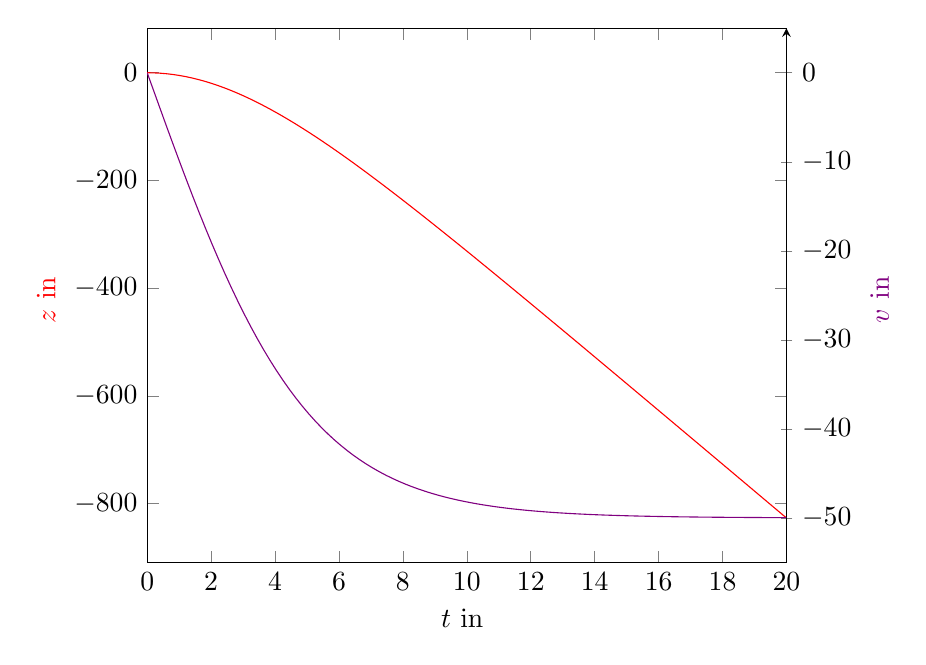
\begin{tikzpicture}[scale = 1, domain = 0:20, samples = 100]
			\begin{axis}[width = 0.8\linewidth, xmin = 0, xmax = 20, xlabel = {$t$ in $\unit{\second}$}, ylabel = {\color{red} $z$ in $\unit{\metre}$}]
				\addplot[mark = none, color = red] (\x,{-(65/0.26)*ln(cosh(-sqrt(0.26*10/65)*\x))});
			\end{axis}
			\begin{axis}[width = 0.8\linewidth, xmin = 0, xmax = 20, ymin = -55, ymax = 5, axis x line = none, axis y line = right, axis y label/.append style = {violet}, ylabel = {\color{violet} $v$ in $\unit{\metre\per\second}$}]
				\addplot[mark = none, color = violet] (\x,{sqrt(65 * 10/0.26)*tanh(-sqrt(0.26*10/65)*\x)});
			\end{axis}
		\end{tikzpicture}
	\item Zeitpunkt zudem sie $95\%$ ihrer Geschwindigkeit erreicht hat:
		\begin{align*}
			t &= \xi \ln \left| \frac{-0.95 \cdot \sqrt{\frac{\frac{\kappa}{F_g}}{\frac{\kappa}{F_g}}} - 1}{-0.95 \cdot \sqrt{\frac{\frac{\kappa}{F_g}}{\frac{\kappa}{F_g}}} + 1}\right| \\
			~ &= \xi \ln \left| \frac{-0.95 - 1}{-0.95 + 1}\right| \\
			~&= \sqrt{\frac{\qty{65}{\kilogram}}{4\cdot\qty{0.26}{\kilogram}\cdot\qty{10}{\metre\per\square\second}}} \ln \left | \frac{ -0.95 - 1}{-0.95 + 1}\right| \\
			t &\approx \qty{9.1589}{\second}
		\end{align*}
		in $ z(t) $ eingesetzt
		\begin{align*}
			z &= - \frac{m}{\kappa} \ln \cosh - \sqrt{-\frac{\kappa a}{m}} t\\
			z &\approx - \frac{\qty{65}{\kilogram}}{\qty{0.26}{\kilogram\per\metre}} \ln \cosh - \sqrt{ \frac{\qty{0.26}{\kilogram\per\metre} \cdot \qty{10}{\metre\per\square\second}}{\qty{65}{\kilogram}}} \qty{9.1589}{\second}\\
			z &\approx \qty{-29e1}{\metre}
		\end{align*}
\end{enumerate}

\section{Zylinderkoordinate}
\begin{enumerate}[label=\alph*)]
	\item $ \rho = \sqrt{ \left(\frac{v_{0,r}}{\omega_c}\right)^2 \sin^2 \omega_c t + \left(\frac{v_{0,r}}{\omega_c}\right)^2 \cos^2 \omega_c t} = \frac{v_{0,r}}{\omega_c} $,\\
		$ \varphi = \arccos \frac{\frac{v_{0,r}}{\omega_c} \cos \omega_c t}{\frac{v_{0,r}}{\omega_c}} = \arccos \cos \omega_c t = \omega_c t $, \\
		$ z = v_{0,z} t $\\
		Die Koordinaten von $ \vec r (t) $ in Zylinderkoordinaten sind also:
		\[ \vec r (t) = \left( \frac{v_{0,r}}{\omega_c}, \omega_c t, v_{0,z} t \right)\]
	\item
		\begin{align*}
			\frac{d}{dt} \vec r &=
			\begin{pmatrix}
				\frac{d\rho}{dt} \cos \varphi - \frac{d\phi}{dt} \rho \sin \varphi\\
				\frac{d\rho}{dt} \sin \varphi + \frac{d\phi}{dt} \rho \cos \varphi\\
				\frac{dz}{dt}
			\end{pmatrix}\\
			\vec v &= 
			\begin{pmatrix}
				- \omega_c \rho \sin \varphi\\
				\omega_c \rho \cos \varphi\\
				v_{0,z}
			\end{pmatrix}
		\end{align*}
		und in Zylinderkoordinaten\\
		$ \rho^\prime = \sqrt{ \left(\omega_c \rho \right)^2 \sin^2 \phi + \left(\omega_c \rho\right)^2 \cos^2 \phi} = \omega_c \rho $,\\
		$ \varphi^\prime = \arccos \frac{-\omega_c \rho}{\rho^\prime} \sin \varphi = \arccos \cos \varphi + \frac{\pi}{2} = \varphi + \frac{\pi}{2} $, \\
		$ z^\prime = v_{0,z} $\\
		also in Zylinderkoordinaten:
		\[ \vec v = \left( \omega_c \rho, \varphi + \frac{\pi}{2}, v_{0,z} \right) = \left( v_{0, r}, \omega_c t + \frac{\pi}{2}, v_{0, z} \right)\]
		\begin{align*}
			\frac{d}{dt} \vec v &=
			\begin{pmatrix}
				\frac{d v_{0, r}}{dt} \cos \omega_c t + \frac{\pi}{2} - \frac{d\omega_c t + \frac{\pi}{2}}{dt} v_{0,r} \sin \omega_c t + \frac{\pi}{2}\\
				\frac{d v_{0, r}}{dt} \sin \omega_c t + \frac{\pi}{2} + \frac{d\omega_c t + \frac{\pi}{2}}{dt} v_{0,r} \cos \omega_c t + \frac{\pi}{2}\\
				\frac{d v_{0,z}}{dt}
			\end{pmatrix}\\
			\vec a &= 
			\begin{pmatrix}
				- \omega_c v_{0, r} \sin \omega_c t + \frac{\pi}{2}\\
				\omega_c v_{0, r} \cos \omega_c t + \frac{\pi}{2}\\
				0
			\end{pmatrix}
		\end{align*}
		Also in Zylinderkoordinaten\\
		$ \rho^{\prime\prime} = \sqrt{ \left(\omega_c v_{0, r} \right)^2 \sin^2 \phi + \left(\omega_c v_{0, r} \right)^2 \cos^2 \phi} = \omega_c v_{0, r}$,\\
		$ \varphi^{\prime\prime} = \arccos \frac{-\omega_c v_{0, r}}{\omega_c v_{0, r}} \sin \omega_c t + \frac{pi}{2} = \arccos \cos \omega_c t + \pi = \omega_c t + \pi $, \\
		$ z^{\prime\prime} = 0 $\\
		Also in Zylinderkoordinaten:
		\[ \vec a = \left( \omega_c v_{0, r}, \omega_c t + \pi, 0 \right) = \left( \omega_c v_{0, r}, - \omega_c t, 0 \right) \]
\end{enumerate}
\end{document}
